\documentclass[tcc,ec]{texfurg} % EC / EA / SI | PPGComp / PPGMC

\usepackage[utf8]{inputenc}     % para acentuação
\usepackage{graphicx}           % para figuras
\usepackage{multirow}           % para tabelas
\usepackage{lipsum}             % lorem ipsum

\title{Modelo TCC para Engenharia de Computação}

\author{UltimoNome}{Nome Sobrenome de}
\advisor[Prof.~Dr.]{Aguiar}{Marilton Sanchotene de}
\coadvisor[Prof.~Dr.]{Gon\c{c}alves}{Eder Mateus Nunes}
\collaborator[Prof.~Dr.]{D'Alessandro}{Andrés Nicolás}

\examiner{Prof.~Dr.~Armando Multas}
\examiner{Prof\textsuperscript{a}.~Dr\textsuperscript{a}.~Nomelinda Longuinha da Silva Paes Netto}
\examiner{Prof.~MSc.~Gerúndio das Dores}


\keyword{palavra um}
\keyword{palavra dois}
\keyword{palavra três}
\keyword{palavra quatro}
% Até 10 palavras chaves


%%%%%%%%%%%%%%%%%%%%%%%%%%%%%%%%%%%%%%%%%%%%%%%%%%%%%%%%%%%%%%%%%%%%%%%%%%%%%%%%
%%%%%%%%%%%%%%%%%%%%%%%%%%%%%%%%%%%%%%%%%%%%%%%%%%%%%%%%%%%%%%%%%%%%%%%%%%%%%%%%


\begin{document}

%\renewcommand{\advisorname}{Orientadora}           % descomente caso tenhas orientadora
%\renewcommand{\coadvisorname}{Co-orientadora}      % descomente caso tenhas co-orientadora

\maketitle

\sloppy

%Resumo em Português.
\begin{abstract}
     Resumo em Português.
\end{abstract}

% Resumo em Inglês
\begin{englishabstract}{English Title}{english, keywords, comma, separated}
    Abstract in English.
\end{englishabstract}

%%%%%%%%%%%%%%%%%%%%%%%%%%%%%%%%%%%%%%%%%%%%%%%%%%%%%%%%%%%%%%%%%%%%%%%%%%%%%%%%

%Lista de Figuras
\listoffigures

%Lista de Tabelas
\listoftables

%lista de abreviaturas e siglas
\begin{listofabbrv}{SPMD}
    \item[ABC] \textit{Abcd Bcde Cdef}
    \item[XYZ] \textit{Xbcd Ycde Zdef}
\end{listofabbrv}

%Sumario
\tableofcontents

  
%%%%%%%%%%%%%%%%%%%%%%%%%%%%%%%%%%%%%%%%%%%%%%%%%%%%%%%%%%%%%%%%%%%%%%%%%%%%%%%%
%%%%%%%%%%%%%%%%%%%%%%%%%%%%%%%%%%%%%%%%%%%%%%%%%%%%%%%%%%%%%%%%%%%%%%%%%%%%%%%%

\chapter{Capítulo Um}

\lipsum[18]

% Ex.: Opcional
\section{Seção Um}

\lipsum[1]

\subsection{Subseção}

\lipsum[2]

\subsubsection{Sub-subseção}

\lipsum[15]

\paragraph{Parágrafo}

\lipsum[17]

%%%%%%%%%%%%%%%%%%%%%%%%%%%%%%%%%%%%%%%%%%%%%%%%%%%%%%%%%%%%%%%%%%%%%%%%%%%%%%%%

\chapter{Capítulo Dois}

O trabalho de \citet{knuth:84} mostrou os fundamentos...

\lipsum[3]

Em \citet{boulic:91} o tempo utilizado para o mesmo experimento foi na ordem de $10^6$ segundos.

\lipsum[6]

Ambos \citep{knuth:84, smith:99} provaram que o protocolo é suscetível a diferentes ataques.

\lipsum[7]

%%%%%%%%%%%%%%%%%%%%%%%%%%%%%%%%%%%%%%%%%%%%%%%%%%%%%%%%%%%%%%%%%%%%%%%%%%%%%%%%

\chapter{Capítulo Três}

Exemplo de figura. A figura~\ref{nome_figura} apresenta.

    \begin{figure}[htbp]
        \centering 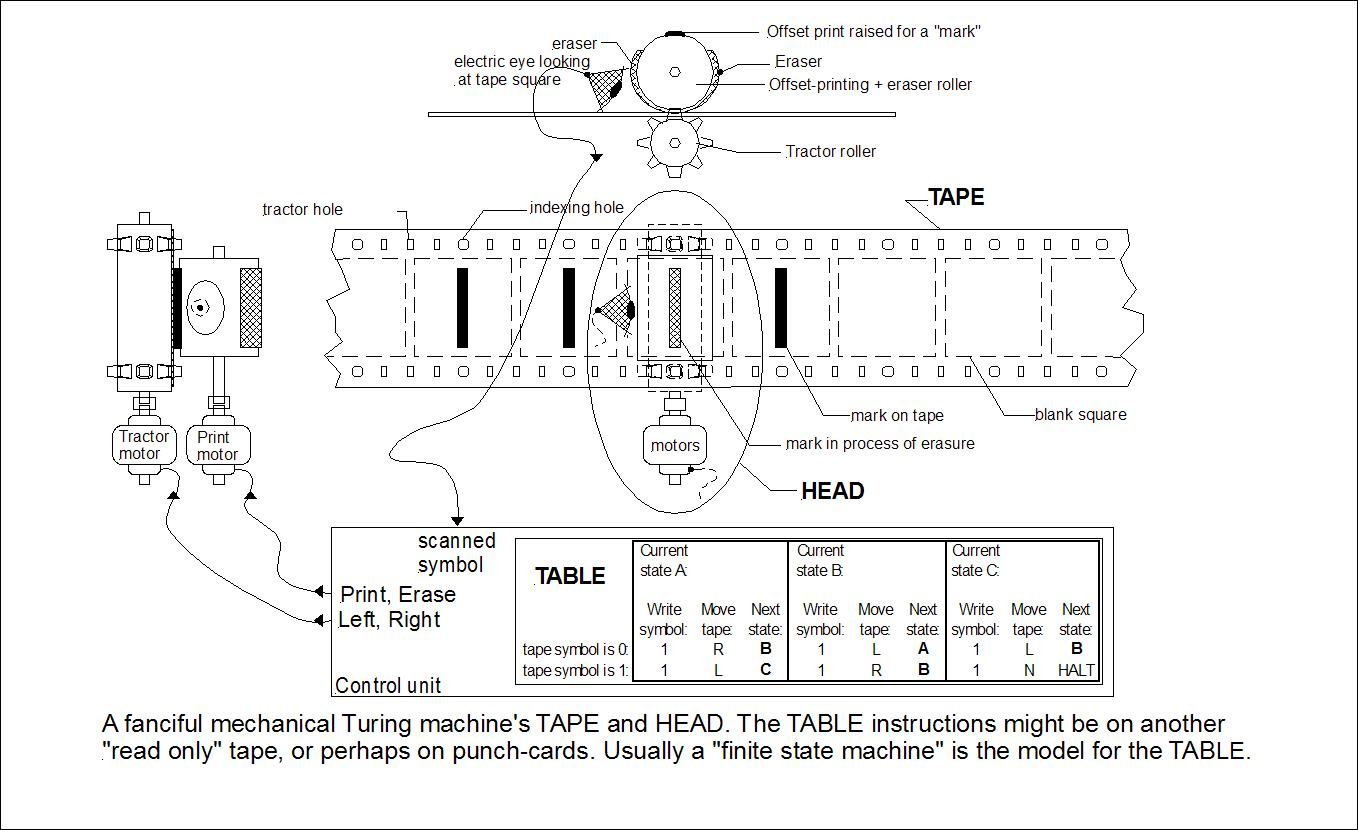
\includegraphics[scale=.3]{turing_machine.eps}
        \caption{Legenda de Figura}
        \label{nome_figura}
    \end{figure}

Exemplo de Tabela. Conforme tabela~\ref{tabela}...

    \begin{table}[htbp]
        \begin{center}
            \caption{Nome da Tabela}
            \label{tabela}
            \begin{tabular}{ccc}
                \hline
                Coluna A & Coluna B & Tempos \\
                \hline
                1       & 2     & 3     \\
                4       & 5     & 6     \\
                7       & 8     & 9     \\
                10      & 11    & 12    \\
                \hline
            \end{tabular}
        \end{center}
    \end{table}

%%%%%%%%%%%%%%%%%%%%%%%%%%%%%%%%%%%%%%%%%%%%%%%%%%%%%%%%%%%%%%%%%%%%%%%%%%%%%%%%
%%%%%%%%%%%%%%%%%%%%%%%%%%%%%%  REFERENZAS  %%%%%%%%%%%%%%%%%%%%%%%%%%%%%%%%%%%%
%%%%%%%%%%%%%%%%%%%%%%%%%%%%%%%%%%%%%%%%%%%%%%%%%%%%%%%%%%%%%%%%%%%%%%%%%%%%%%%%

\bibliography{mendeley_v2}
\bibliographystyle{abnt}

% Anexos (Opcional)
\annex
\chapter{Um exemplo de anexo}

\lipsum[10-12]

\chapter{Outro anexo exemplo}

\lipsum[13-14]

\end{document}